\section{Experimentos y análisis de resultados}
	
	\subsection{Procedimiento de desarrollo de la práctica}
	
	\paragraph{}Para realizar la práctica, se ha optado por implementar las heurísticas propuestas en el lenguaje de programación \textsc{Java}. El ejecutable que se entrega junto a este documento ha sido compilado bajo \textsc{ Apache NetBeansIDE 12.0}.
	
	\subsubsection{Equipo de pruebas}
	
	\paragraph{}Los resultados de las heurísticas han sido obtenidos en el siguiente equipo:
	
		\begin{itemize}
			
			\item Host:
			\item S.O:
			\item Kernel:
			\item CPU:
			\item GPU:
			\item GPU:
			\item Memoria RAM :
			
		\end{itemize}

	\subsubsection{Manual de usuario}
	
		\paragraph{}Para ejecutar el software asegúrese de que el archivo .jar proporcionado se ubica en el mismo directorio que la carpeta \emph{archivos}. 
		
		\paragraph{}Cuando se muestre la GUI, podrá seleccionar la heurística que desee mediante el botón correspondiente. Una vez empiece la ejecución de una heurística no sera posible seleccionar otra hasta que finalice su ejecución. Los resultados finales se mostrarán en el cuadro de texto, a su vez, se generan los log correspondientes a cada archivo y semilla en la carpeta Log.
	
		\begin{figure}[H]
		
			\centering
			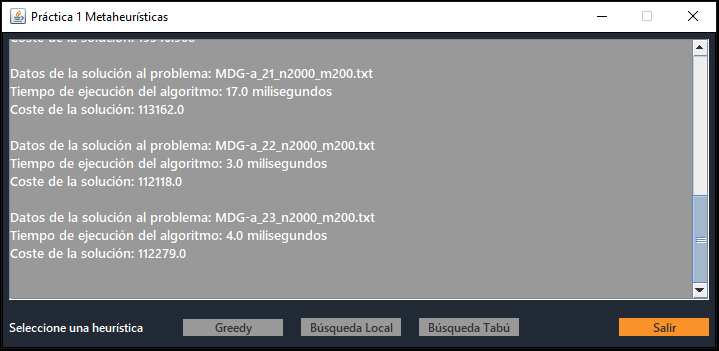
\includegraphics[scale=0.4]{img/GUI}
			\caption{GUI}
		
		\end{figure}
	
	\subsection{Parámetros de los algoritmos}
	
		\subsubsection{Sistema de Colonias de Hormigas}

		\paragraph{}Para regular el comportamiento del Sistema de Colonias de Hormigas, se han definido los siguientes parámetros en el archivo de configuración:
		
		\begin{itemize}
			
			\item Iteraciones:  Número máximo de iteraciones realizadas por el algoritmo principal, valor por defecto: 10.000.
			\item Número de hormigas: Número de hormigas pertenecientes a cada colonia generada en cada iteración, valor por defecto: 10.
			\item Q0: Probabilidad de no elegir directamente el candidato que mayor coste aporta a la hormiga en la regla de la transición, valor por defecto: 0,95.
			\item Beta: Exponente aplicado al coste de los arcos en las fórmulas de la regla de la transición, valores por defecto: 1 y 2.
			\item Alfa: Exponente aplicado a la feromona de los arcos en las fórmulas de la regla de la transición, valores por defecto: 1 y 2.
			\item Rho: Constante aplicada en la fórmula de la evaporación global de feromona, valor por defecto: 0,1.
			\item Phi: Constante aplicada en la fórmula de la evaporación local de feromona, valor por defecto: 0,1.
			\item Delta: Porcentaje de restricción aplicado sobre la lista de candidatos total de una hormiga, valor por defecto: 0,75.
			
		\end{itemize}
	\subsubsection{Semillas}
	
	\paragraph{}Para la generación de números pseudoaleatorios se utiliza una semilla previamente definida en el archivo de configuración, en este caso es 77356084. Esta semilla se va rotando en las 5 iteraciones de cada archivo.
	
	
	\paragraph{} 77356084 $\rightarrow$ 73560847 $\rightarrow$ 35608477  ...
	
	
	\subsection{Análisis de los resultados}
	
		\subsubsection{SCH con $\alpha$ = 1, $\beta$ =1}
		
		\begin{table}[H]
			\begin{center}
				\begin{tabular}{| c | c | c | c | c | c | c |}
					\hline
					\multicolumn{7}{ |c| }{SCH $\alpha$ = 1, $\beta$ =1} \\ \hline
					& \multicolumn{2}{ |c| }{GKD-c\_1\_n500\_m50} & \multicolumn{2}{ |c| }{GKD-c\_2\_n500\_m50} & \multicolumn{2}{ |c| }{GKD-c\_3\_n500\_m50} \\ \hline
					Ejecución & Coste & Tiempo & Coste & Tiempo & Coste & Tiempo \\ \hline
					1 &19447,05 & 86283 & 19677,01 & 85025 & 19525,05 & 85636\\
					2 &19460,39 & 85767 & 19674,26 & 85178 & 19523,76 & 85188\\
					3 &19462,50	& 87097 & 19670,57 & 85011 & 19519,77 & 85287\\
					4 &19458,63	& 86364 & 19661,08 & 85106 & 19523,81 & 85303\\
					5 &19462,67 & 86277 & 19674,56 & 85214 & 19531,01 & 85232\\ \hline
					Media & -0,14\% & 86357,60 & -0,15\% & 85106,80 & -0,12\% & 85329,20\\ \hline
					Devs. típica & 0,03\% & 476,35 & 0,03\% & 90,04 & 0,02\% & 177,47 \\ \hline
				\end{tabular}
				\caption{Resultados GKD}
				\label{tab:tabalfa1beta1GKD}
			\end{center}
		\end{table} 
		
		
		\begin{table}[H]
			\begin{center}
				\begin{tabular}{| c | c | c | c | c | c | c |}
					\hline
					\multicolumn{7}{ |c| }{SCH $\alpha$ = 1, $\beta$ =1} \\ \hline
					& \multicolumn{2}{ |c| }{SOM-b\_11\_n300\_m90} & \multicolumn{2}{ |c| }{SOM-b\_12\_n300\_m120} & \multicolumn{2}{ |c| }{SOM-b\_13\_n400\_m40} \\ \hline
					Ejecución & Coste & Tiempo & Coste & Tiempo & Coste & Tiempo\\\hline
					1 &20662 & 167862 & 35800 & 263791 & 4630 & 53726\\
					2 &20658 & 167622 & 35793 & 264292 & 4626 & 53753\\
					3 &20645 & 167410 & 35780 & 263622 & 4646 & 53726\\
					4 &20623 & 167560 & 35828 & 263551 & 4631 & 53832\\
					5 &20634 & 167525 & 35776 & 263251 & 4629 & 54074\\\hline
					Media &-0,48\% & 167595,80 & -0,24\% & 263701,40 & -0,55\% & 604,40\\ \hline
					Devs. típica & 0,08\% & 167,70 & 0,06\% & 383,61 & 0,17\% & 7,44 \\ \hline
				\end{tabular}
				\caption{Resultados SOM}
				\label{tab:tabalfa1beta1SOM}
			\end{center}
		\end{table} 
		
		\begin{table}[H]
			\begin{center}
				\begin{tabular}{| c | c | c | c | c | c | c |}
					\hline
					\multicolumn{7}{ |c| }{SCH $\alpha$ = 1, $\beta$ =1} \\ \hline
					& \multicolumn{2}{ |c| }{MDG-a\_21\_n2000\_m200} & \multicolumn{2}{ |c| }{MDG-a\_22\_n2000\_m200} & \multicolumn{2}{ |c| }{MDG-a\_23\_n2000\_m200}\\\hline
					Ejecución & Coste & Tiempo & Coste & Tiempo & Coste & Tiempo\\\hline
					1 &113383,00 & 600256,00 & 113153,00 & 600090,00 & 113132,00 & 600032,00\\
					2 &113539,00 & 600065,00 & 113180,00 & 600185,00 & 113110,00 & 600298,00\\
					3 &113368,00 & 600107,00 & 113439,00 & 600184,00 & 113088,00 & 600292,00\\
					4 &113483,00 & 600283,00 & 113232,00 & 600161,00 & 113064,00 & 600116,00\\
					5 &113307,00 & 600149,00 & 113258,00 & 600124,00 & 113085,00 & 600223,00\\\hline
					Media &-0,74\% & 600172,00 & -0,94\% & 600178,80 & -0,90\% & 6000192,20\\ \hline
					Devs. típica & 0,08\% & 94,31 & 0,10\% & 41,14 & 0,02\% & 115,73 \\ \hline
				\end{tabular}
				\caption{Resultados MDG}
				\label{tab:tabalfa1beta1MDG}
			\end{center}
		\end{table}
		
		\paragraph{} Como puede observarse en los resultados, el algoritmo exhibe un comportamiento robusto, manteniendo las desviación típica de los resultados por debajo del 0,20\% en todos los archivos de datos estudiados. Si evaluamos la calidad de las soluciones obtenidas respecto a costes, el algoritmo es incapaz de encontrar los óptimos globales con los parámetros anteriormente descritos.
		
		\paragraph{} En lo referente a tiempos, el algoritmo consigue ejecutar las iteraciones objetivo antes de los 600 segundos para las instancias pequeñas y medianas. No es el caso de las instancias de datos más grandes, dónde el algoritmo finaliza su ejecución en torno las 2000 iteraciones. 
		
		\subsection{SCH con $\alpha$ = 2, $\beta$ =1}
		
		\subsection{SCH con $\alpha$ = 1, $\beta$ =2}
	
		\begin{table}[H]
			\begin{center}
				\begin{tabular}{| c | c | c | c | c | c | c |}
					\hline
					\multicolumn{7}{ |c| }{SCH $\alpha$ = 1, $\beta$ =1} \\ \hline
					& \multicolumn{2}{ |c| }{GKD-c\_1\_n500\_m50} & \multicolumn{2}{ |c| }{GKD-c\_2\_n500\_m50} & \multicolumn{2}{ |c| }{GKD-c\_3\_n500\_m50} \\ \hline
					Ejecución & Coste & Tiempo & Coste & Tiempo & Coste & Tiempo \\ \hline
					1 &19458,15 & 77625,00 & 19671,65 & 74997,00 & 19524,13 & 75122,00\\
					2 &19464,52 & 75155,00 & 19674,24 & 75196,00 & 19517,79 & 75309,00\\
					3 &19461,56	& 75467,00 & 19672,58 & 75163,00 & 19512,71 & 75040,00\\
					4 &19453,08	& 76501,00 & 19663,09 & 75141,00 & 19519,27 & 75298,00\\
					5 &19455,44 & 75050,00 & 19671,50 & 75515,00 & 19513,44 & 75086,00\\ \hline
					Media & -0,14\% & 75959,60 & -0,16\% & 75202,40 & -0,15\% & 75171,00\\ \hline
					Devs. típica & 0,02\% & 1093,63& 0,02\% & 190,57 & 0,02\% & 124,46\\ \hline
				\end{tabular}
				\caption{Resultados GKD}
				\label{tab:tabalfa1beta2GKD}
			\end{center}
		\end{table} 
		
		
		\begin{table}[H]
			\begin{center}
				\begin{tabular}{| c | c | c | c | c | c | c |}
					\hline
					\multicolumn{7}{ |c| }{SCH $\alpha$ = 1, $\beta$ =1} \\ \hline
					& \multicolumn{2}{ |c| }{SOM-b\_11\_n300\_m90} & \multicolumn{2}{ |c| }{SOM-b\_12\_n300\_m120} & \multicolumn{2}{ |c| }{SOM-b\_13\_n400\_m40} \\ \hline
					Ejecución & Coste & Tiempo & Coste & Tiempo & Coste & Tiempo\\\hline
					1 &20622,00 & 139098,00 & 35778,00 & 213206,00 & 4623,00 & 47794,00\\
					2 &20642,00 & 138657,00 & 35788,00 & 213358,00 & 4625,00 & 47931,00\\
					3 &20626,00 & 139174,00 & 35801,00 & 213563,00 & 4645,00 & 47870,00\\
					4 &20630,00 & 139116,00 & 35798,00 & 213505,00 & 4628,00 & 48003,00\\
					5 &20659,00 & 139407,00 & 35777,00 & 213245,00 & 4630,00 & 48161,00\\\hline
					Media &-0,52\% & 139090,40 & -0,26\% & 213375,40 & -0,60\% & 47951,80\\ \hline
					Devs. típica & 0,07\% & 271,93 & 0,03\% & 156,52 & 0,19\% & 140,01\\ \hline
				\end{tabular}
				\caption{Resultados SOM}
				\label{tab:tabalfa1beta2SOM}
			\end{center}
		\end{table} 
		
		\begin{table}[H]
			\begin{center}
				\begin{tabular}{| c | c | c | c | c | c | c |}
					\hline
					\multicolumn{7}{ |c| }{SCH $\alpha$ = 1, $\beta$ =1} \\ \hline
					& \multicolumn{2}{ |c| }{MDG-a\_21\_n2000\_m200} & \multicolumn{2}{ |c| }{MDG-a\_22\_n2000\_m200} & \multicolumn{2}{ |c| }{MDG-a\_23\_n2000\_m200}\\\hline
					Ejecución & Coste & Tiempo & Coste & Tiempo & Coste & Tiempo\\\hline
					1 &113382,00 & 600068,00 & 113280,00 & 600167,00 & 113246,00 & 600160,00\\
					2 &113460,00 & 600100,00 & 113189,00 & 600228,00 & 113009,00 & 600159,00\\
					3 &113257,00 & 600161,00 & 113464,00 & 600081,00 & 113136,00 & 600202,00\\
					4 &113281,00 & 600139,00 & 113209,00 & 600100,00 & 113153,00 & 600118,00\\
					5 &113376,00 & 600014,00 & 113202,00 & 600126,00 & 113109,00 & 600223,00\\\hline
					Media &-0,79\% & 600096,40 & -0,93\% & 600140,40 & -0,87\% & 6000174,40\\ \hline
					Devs. típica & 0,07\% & 58,30 & 0,10\% & 58,63 & 0,07\% & 44,22 \\ \hline
				\end{tabular}
				\caption{Resultados MDG}
				\label{tab:tabalfa1beta2MDG}
			\end{center}
		\end{table}

	\subsection{Evolución de los resultados}
	
	\begin{figure}[H]
		\centering
		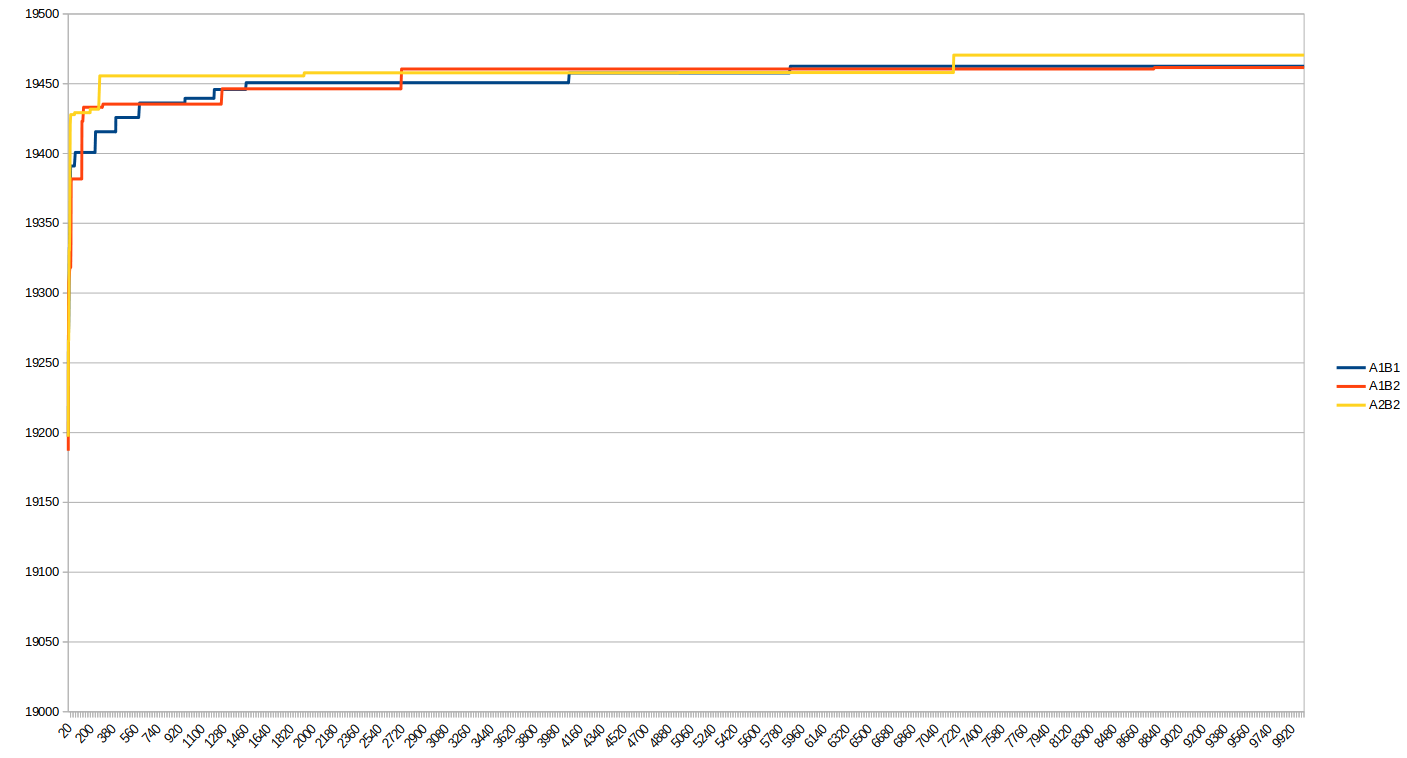
\includegraphics[scale=0.3]{img/GKD1conver.png}
		\caption{Evolución del mejor coste en la ejecución de todos los algoritmos respecto al número de evaluaciones para el problema GKD-c1, semilla 35608477}
		\label{gkd-c1_historico}
	\end{figure}

	\begin{figure}[H]
		\centering
		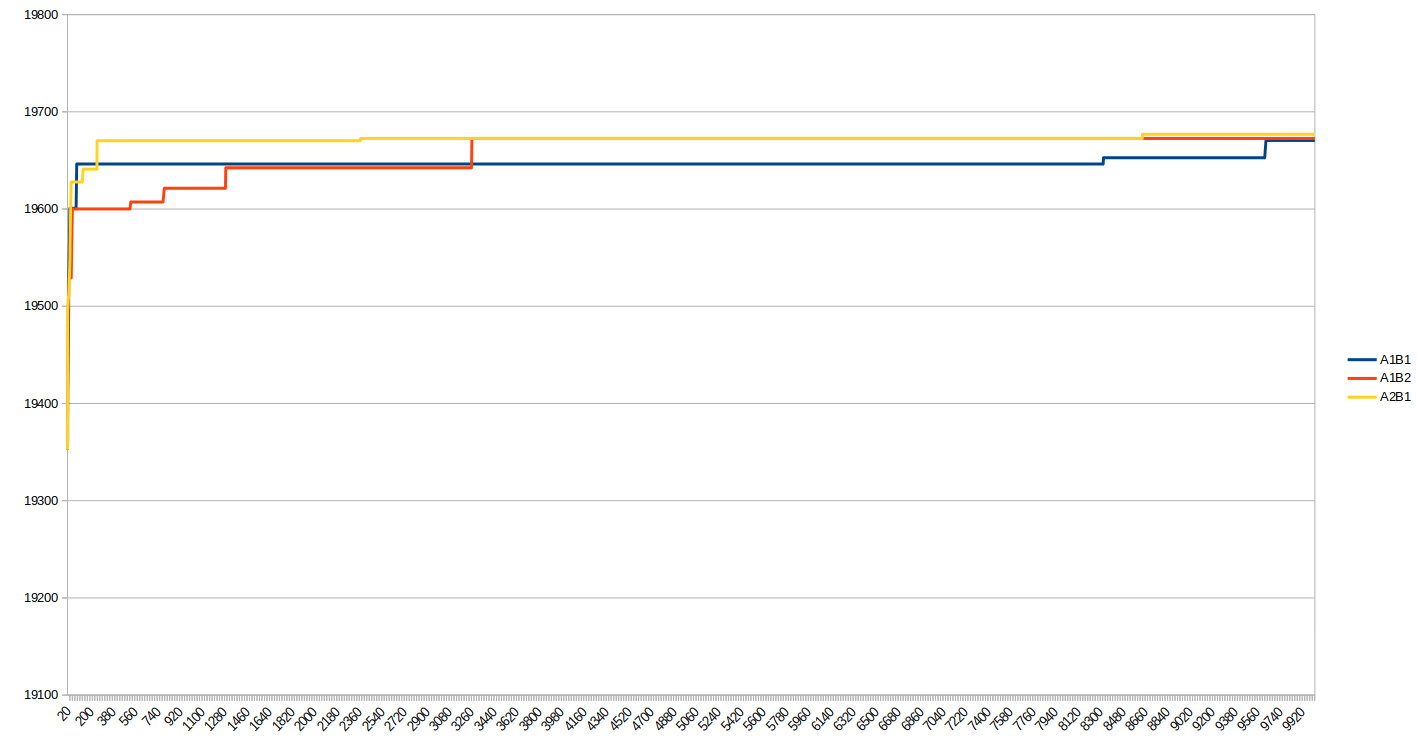
\includegraphics[scale=0.3]{img/GKD2conver.png}
		\caption{Evolución del mejor coste en la ejecución de todos los algoritmos 	respecto al número de evaluaciones para el problema GKD-c1, semilla 35608477}
		\label{gkd-c2_historico}
	\end{figure}

	\begin{figure}[H]
		\centering
		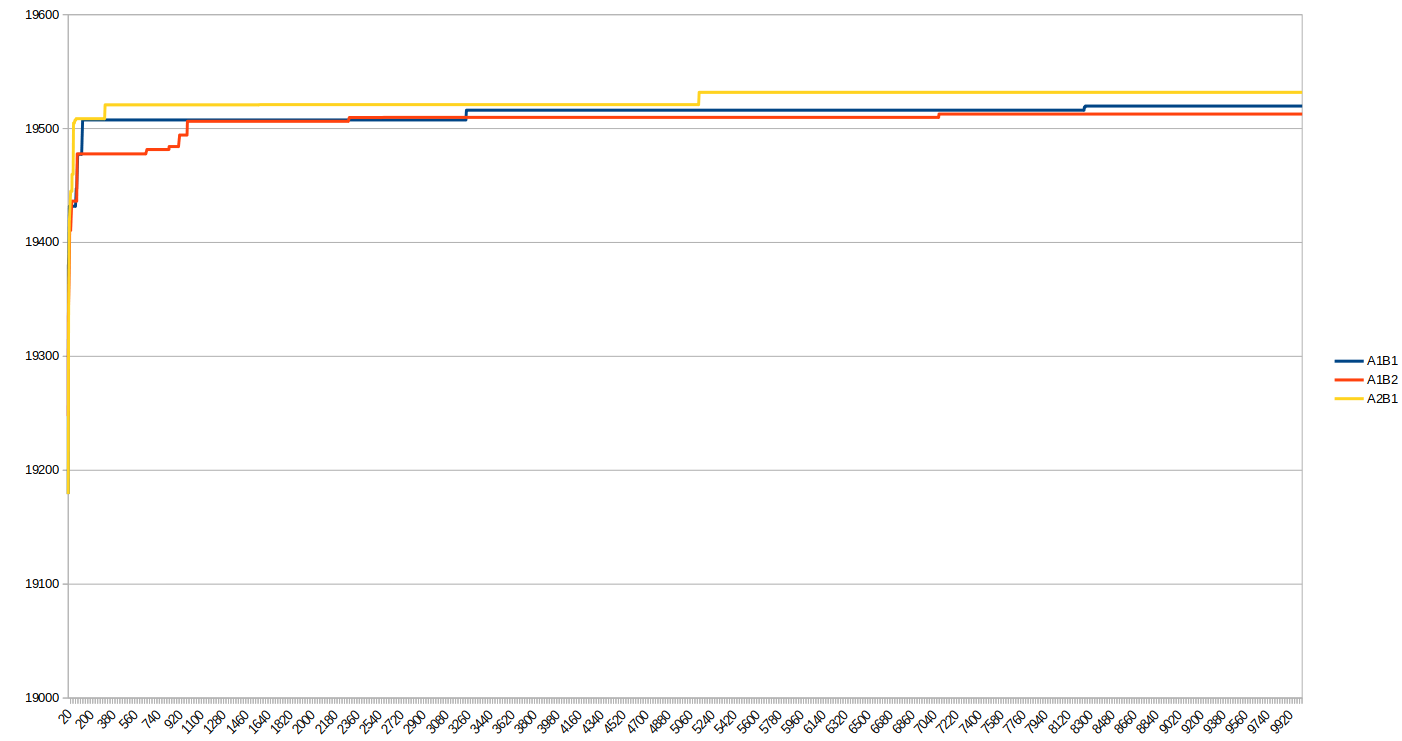
\includegraphics[scale=0.3]{img/GKD3conver.png}
		\caption{Evolución del mejor coste en la ejecución de todos los algoritmos respecto al número de evaluaciones para el problema GKD-c1, semilla 35608477}
		\label{gkd-c3_historico}
	\end{figure}

	\begin{figure}[H]
		\centering
		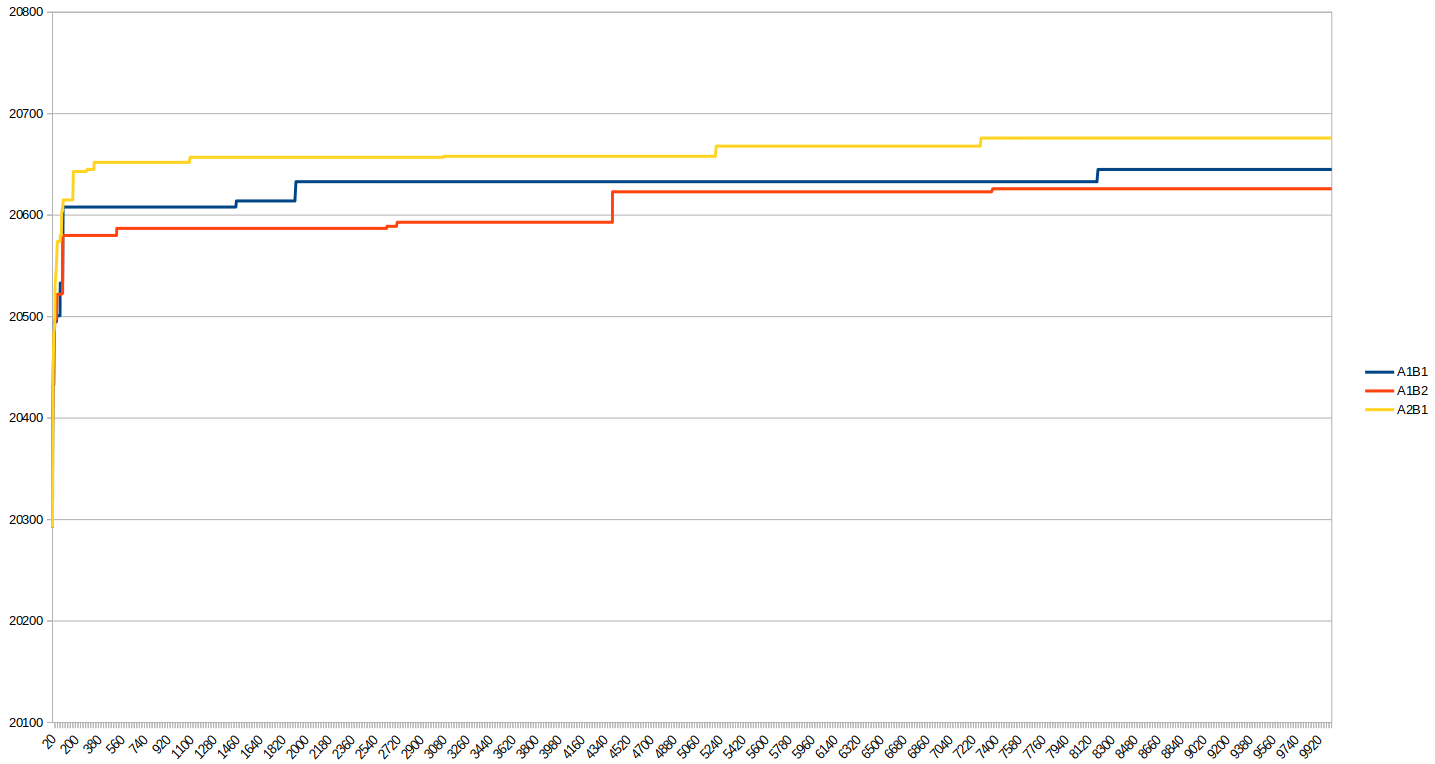
\includegraphics[scale=0.3]{img/SOM1conver.png}
		\caption{Evolución del mejor coste en la ejecución de todos los algoritmos respecto al número de evaluaciones para el problema GKD-c1, semilla 35608477}
		\label{SOM-b_11_historico}
	\end{figure}

	\begin{figure}[H]
		\centering
		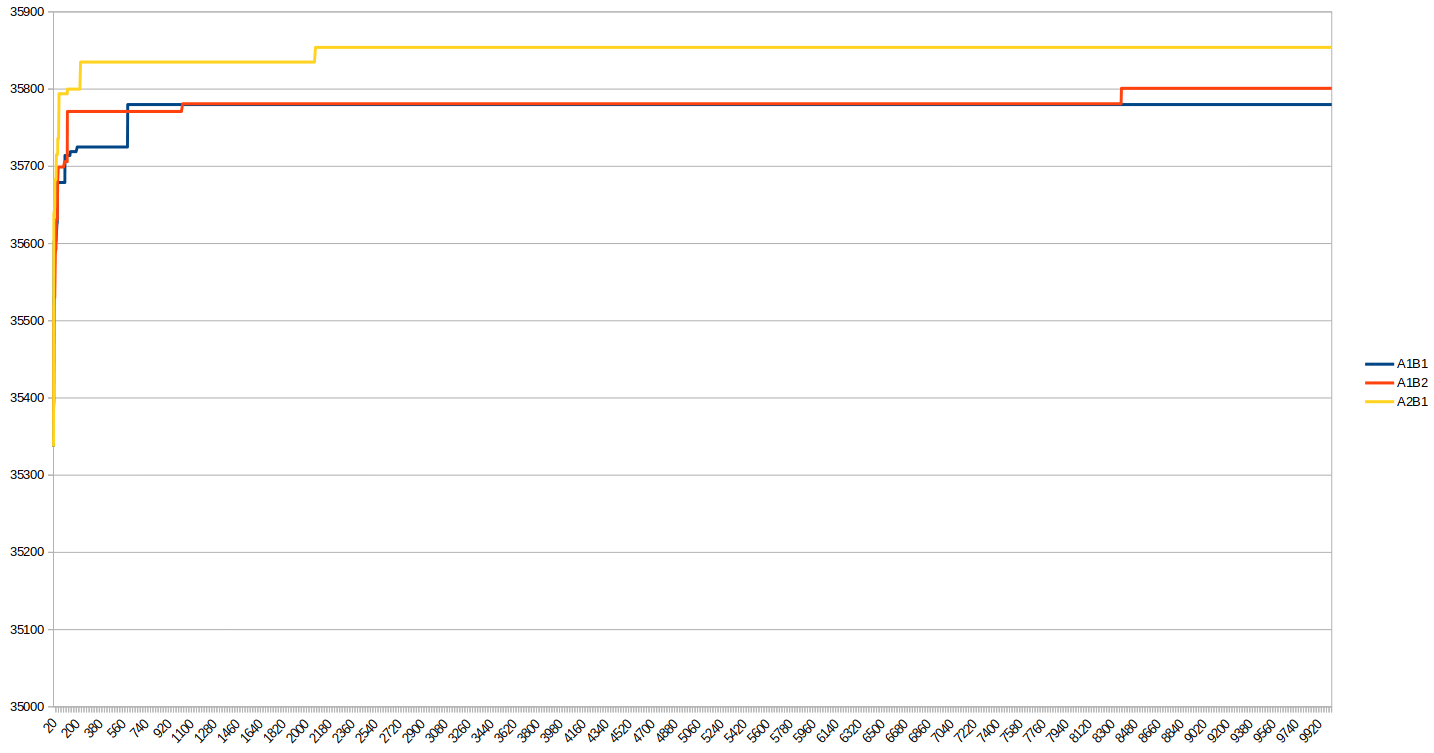
\includegraphics[scale=0.3]{img/SOM2conver.png}
		\caption{Evolución del mejor coste en la ejecución de todos los algoritmos respecto al número de evaluaciones para el problema GKD-c1, semilla 35608477}
		\label{SOM-b_12_historico}
	\end{figure}

	\begin{figure}[H]
		\centering
		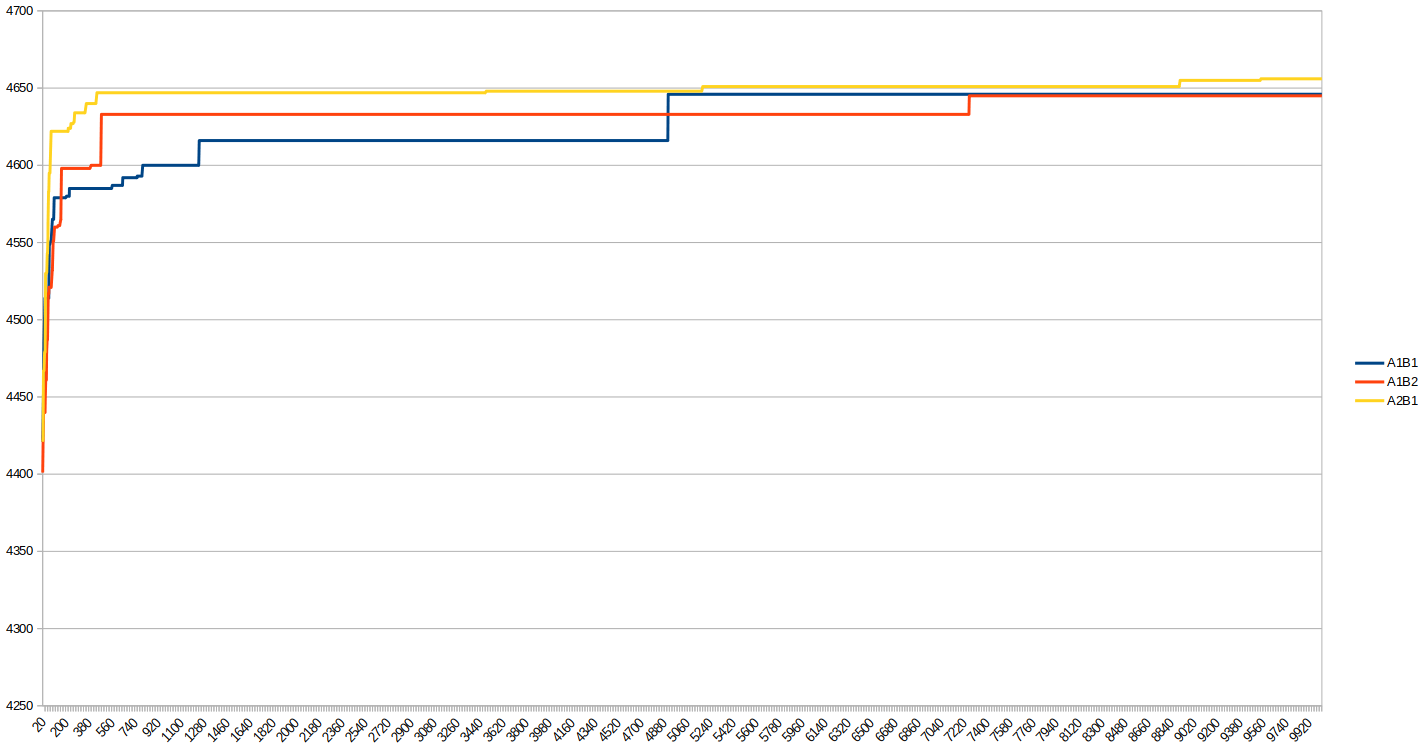
\includegraphics[scale=0.3]{img/SOM3conver.png}
		\caption{Evolución del mejor coste en la ejecución de todos los algoritmos respecto al número de evaluaciones para el problema GKD-c1, semilla 35608477}
		\label{SOM-b_13_historico}
	\end{figure}

	\begin{figure}[H]
		\centering
		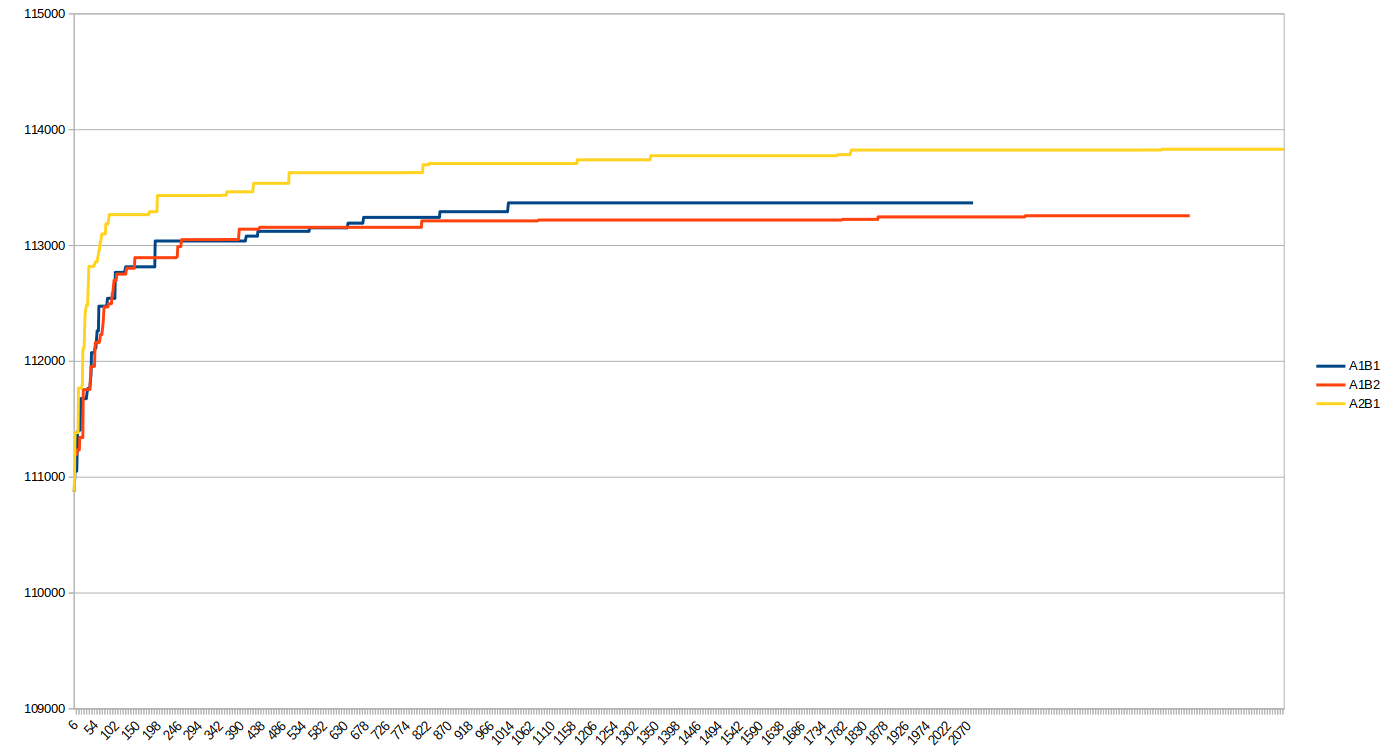
\includegraphics[scale=0.3]{img/MDG1conver.png}
		\caption{Evolución del mejor coste en la ejecución de todos los algoritmos respecto al número de evaluaciones para el problema GKD-c1, semilla 35608477}
		\label{MDG-a_21_historico}
	\end{figure}

	\begin{figure}[H]
		\centering
		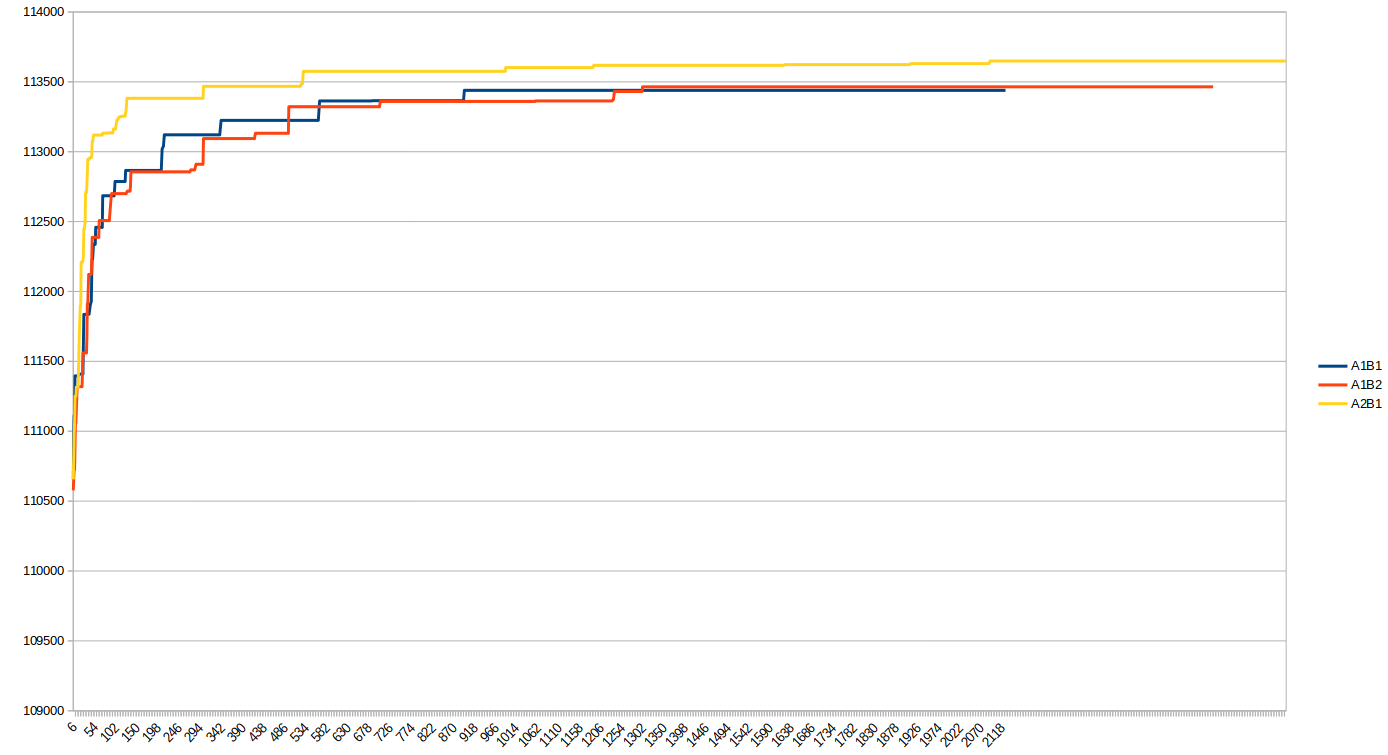
\includegraphics[scale=0.3]{img/MDG2conver.png}
		\caption{Evolución del mejor coste en la ejecución de todos los algoritmos respecto al número de evaluaciones para el problema GKD-c1, semilla 35608477}
		\label{MDG-a_22_historico}
	\end{figure}

	\begin{figure}[H]
		\centering
		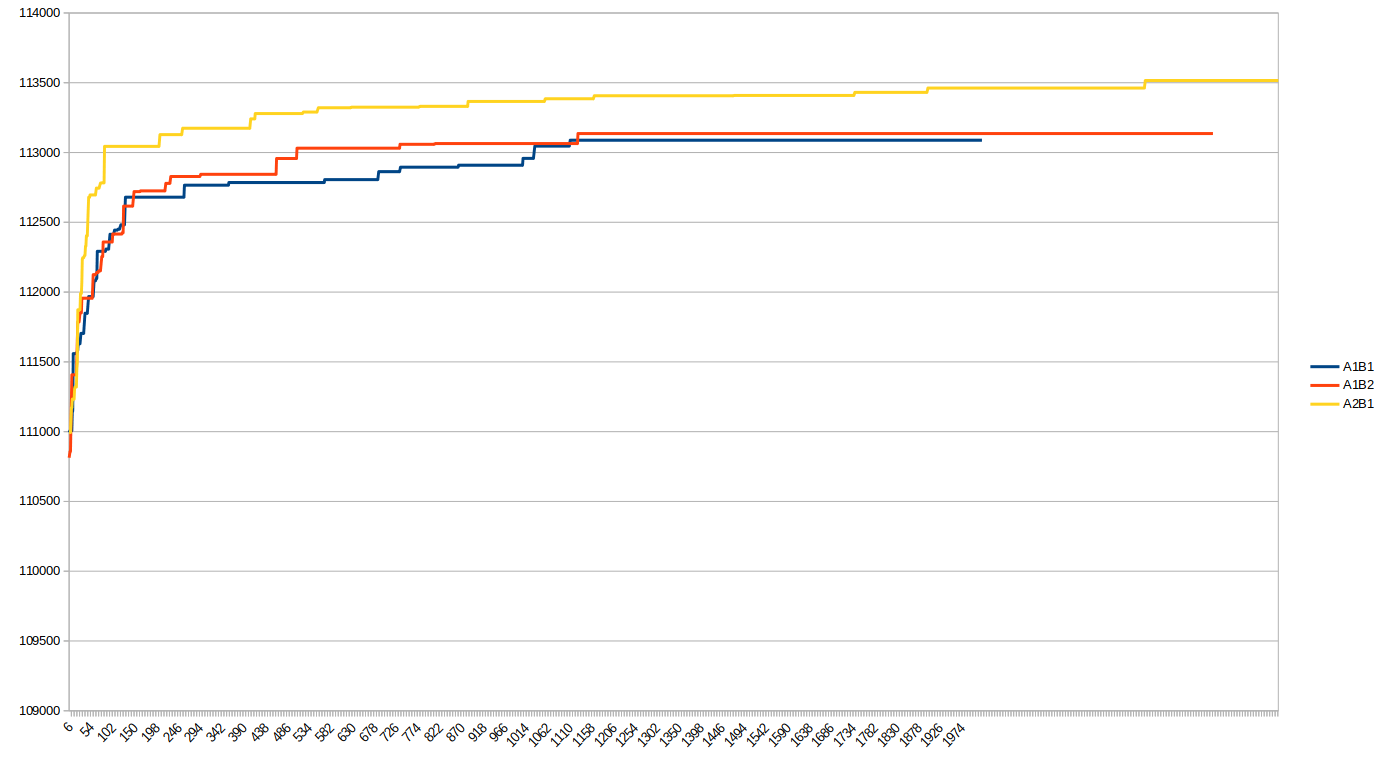
\includegraphics[scale=0.3]{img/MDG3conver.png}
		\caption{Evolución del mejor coste en la ejecución de todos los algoritmos respecto al número de evaluaciones para el problema GKD-c1, semilla 35608477}
		\label{MDG-a_23_historico}
	\end{figure}